\section{Klassifikation mit Entscheidungsbäumen}

\subsection{Attribute vs. Features}
Im Folgenden sei unser Trainingsdatenbestand \(T\) beschrieben durch
\[
	T = \{ (A, l_i) \}
\]
wobei \(A\) eine Menge von Attributen und \(l_i \in L\) ein Label / die
Klassenzugehörigkeit des Datenobjektes ist. Betrachten wir nun als Beispiel
die Daten der Überwachung eines Schiffsmotors hinsichtlich der Temperaturen.
So könnte man die Temperaturen zu unterschiedlichen Zeiten messen, um daraus
zwei Klassen "'Motor läuft in 5 Minuten noch"' und "'Motor ist in 5 Minuten
kaputt"' zu bilden. Wenn nun eine neue Temperaturmessung erfolgt, soll also
vorhergesagt werden, wie der Status des Motors in 5 Minuten sein wird.
Dabei sind die einzelnen Temperaturen an sich jedoch nicht sonderlich aussagekräftig.
Es wäre z.B. viel interessanter zu wissen, ob baugleiche Zylinder zum selben
Zeitpunkt sehr unterschiedliche Temperaturen aufweisen, was auf eine Fehlfunktion
hinweisen kann. Auch der Temperaturanstieg innerhalb der letzten 5 Minuten wäre
interessant zu wissen. Abstrakt handelt es sich hierbei um Funktionen, die 
die Attribute auf andere Werte abbilden. Diese Werte sind die sogenannten
\textit{Features} (Merkmale). Es sind also diese Features, die für die Klassifikation
neuer Messungen wichtig sind.
Angenommen \(\lvert A\rvert = 2\) o.B.d.A.; damit ergibt sich unser neuer Trainingsdatenbestand
\(T'\) zu
\[
	T' = \{ (f_1(x_1,y_1), \dots, f_m(x_1,y_1)), (f_1(x_2,y_2), \dots, f_m(x_2,y_2)), \dots\}
\]
wobei \(f_i\) das \(i\)-te Feature ist.

\subsection{Binäre Entscheidungsbäume}
Ein einfaches Mittel zur Klassifikation sind binäre Entscheidungsbäume. Basierend
auf dem Trainingsdatenbestand wird der Baum erstellt, wobei in den Knoten jeweils
eine Abfrage an die Attribute oder Features erfolgt. Am Ende muss jedes Datenobjekt
auf eines der Blätter abgebildet werden können. Hat man dies getan, wird die 
Klassenzugehörigkeit des Blattes durch das größte Klassenvorkommen der auf das
Blatt abgebildeten Datenobjekte bestimmt.

\begin{figure}[ht]
	\centering
	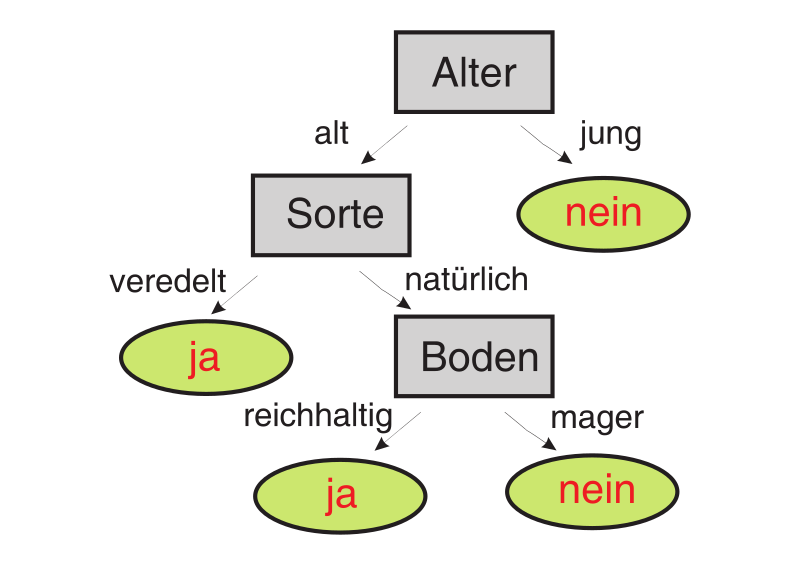
\includegraphics[width=0.75\textwidth]{Figures/decision_tree}
	\caption[Entscheidungsbaum Beispiel]{Beispielhafter Entscheidungsbaum über die
	voraussichtliche Fruchtbarkeit eines Apfelbaumes.\footnotemark}
	\label{fig:decision_tree}
\end{figure}
\footnotetext{https://upload.wikimedia.org/wikipedia/de/6/63/Entscheidungsbaum.svg}

Es spielt eine wichtige Rolle, wie die Splitwerte in den einzelnen Knoten gewählt
werden, da es sonst zu einem Baum kommen könnte, in dem jedes Blatt seine 
Klassenzugehörigkeit nur mit sehr geringem Vorsprung erhalten hat. Hier hilft
uns das Konzept der Entropie weiter: Die Splitwerte werden am besten so gewählt, dass die
Entropie möglichst gering ausfällt, da dann die Heterogenität der Verteilung der
Datenobjekte auf die Blätter am größten ist, der Baum also zutreffendere Vorhersagen
erstellen kann. Hierfür sei
\[
	E(S_1, S_2) = \frac{n_1}{n} E(S_1) + \frac{n_2}{n} E(S_2)
\]
die \textbf{Entropie des Splits}. Hierbei werden also die Entropien der beiden
Teile gewichtet aufsummiert; \(n\) ist die Anzahl der Datenobjekte.

Ein grundlegendes Problem beim algorithmischen Erstellen eines Entscheidungsbaums
ist das so genannte \textbf{Overfitting}. Hierbei werden so lange neue
Entscheidungsregeln erstellt, bis der Fehler bei der Klassifikation des
Trainingsdatenbestandes minimal wird, was jedoch zu einer Erhöhung der Fehlerrate
bei den echten Datenbeständen führen kann. Der Entscheidungsbaum ist also so
speziell an den Trainingsdatenbestand angepasst, dass er schon keine anderen Daten
mehr richtig klassifizieren kann. Es kann also nötig sein, den "'Entscheidungsbaum
ein wenig zu stutzen"', was auf Neudeutsch "'\textbf{Pruning}"' genannt wird. Hierbei
kann im Wesentlichen zwischen zwei Methoden unterschieden werden.

Beim \textbf{Pre-Pruning} wird das "'Wachsen"' des Baumes verhindert, indem bei der
Erstellung der Kindknoten geprüft wird, wie viel der Split einer weiteren Dimension
noch bringt. 

Bei der gängigeren Variante, dem \textbf{Post-Pruning} wird zunächst der gesamte
Entscheidungsbaum aufgebaut, und danach "'zurückgeschnitten"'. Hierfür ist es
zunächst notwendig, den verfügbaren Datenbestand in einen Trainingsteil und einen
Testteil zu unterteilen. Mit dem Trainingsteil wird zunächst der Baum komplett
aufgebaut, danach wird die Fehlerrate anhand des Testbestandes gemessen. Nun wird
sukzessiv ein Knoten nach dem anderen entfernt und jeweils die neue Fehlerrate mit den
Testdaten bestimmt. Die Knoten, deren Entfernung zu einem Sinken der Fehlerrate führen,
werden damit endgültig ausgeschlossen. Dies wird so lange durchgeführt, bis keine
Verbesserung der Fehlerrate mehr feststellbar ist. Dieses Verfahren erzeugt im
Allgemeinen die kleinste Version des Entscheidungsbaumes, benötigt jedoch immer
einen Testdatenbestand.

Anstelle von einer klaren Klasseneinteilung der Blätter ist es im Allgemeinen
nützlicher, stattdessen mit Wahrscheinlichkeiten zu arbeiten. So könnte in
einem Entscheidungsbaum in den Blätter statt den Klassen eher die Wahrscheinlichkeit
der Zugehörigkeit zu einer Klasse angegeben werden, wenn ein Objekt nach Traversieren
des Baumes an diesem Blatt ankommt. Hierfür kann die relative Häufigkeit der 
häufigsten Klasse des Blattes genommen werden. Dies Vorgehen ist jedoch
im Allgemeinen statistisch wenig signifikant und sollte mit Mitteln, die in 
späteren Kapiteln vorgestellt werden, ergänzt werden.

\subsection{Kosten beim Lernen}
Es gibt im Grunde zwei Fehlerarten, die auftreten können: \textbf{False Positives} 
und \textbf{False Negatives}. Im Anwendungskontext ist es oft der Fall, dass der
eine Fehler schlimmere Folgen nach sich zieht als der andere. So kann im 
Bankenwesen bei der Bewertung der Kreditwürdigkeit von Kunden ein False Positive
(Classifier sagt "'Guter Kunde"', obwohl Kunde in Wirklichkeit kreditunwürdig ist)
zu viel höheren Verlusten führen, als ein False Negative (Missed chance). Salopp
formuliert sollte ein Classifier in diesem Kontext also genau darauf achten,
wann er "'Guter Kunde"' voraussagt.

Gegeben einen Entscheidungsbaum mit 2 Klassen \texttt{YES} und \texttt{NO}. Ein
False Positive sei nun ein sehr teurer Fehler (Faktor 10). Dann wollen wir unseren
Entscheidungsbaum besonders darauf trainieren, \texttt{NO}-Objekte richtig zu
identifizieren. Dies kann nun dadurch erreicht werden, dass es 10-mal mehr 
\texttt{NO}-Instanzen in unserem Trainingsdatenbestand gibt als \texttt{YES}-Instanzen.

Eine andere Möglichkeit, Kosten einzusparen, besteht darin, Wahrscheinlichkeiten
zu verwenden. Liefert unser Classifier nun beispielsweise mit \(70\%\) ein
\texttt{NO} für ein \texttt{NO}-Objekt, während die Kosten für ein False Positive 10 betragen,
dann ergeben sich die erwarteten Kosten zu \(0.3 * 10 = 3\) für diese Art von
Fehler. Mit dieser Darstellung
lässt sich nun auch beobachten, dass das wahrscheinlichste Ergebnis nicht auch
die beste Wahl für die Klassifikation ist.

\begin{figure}[ht]
	\centering
	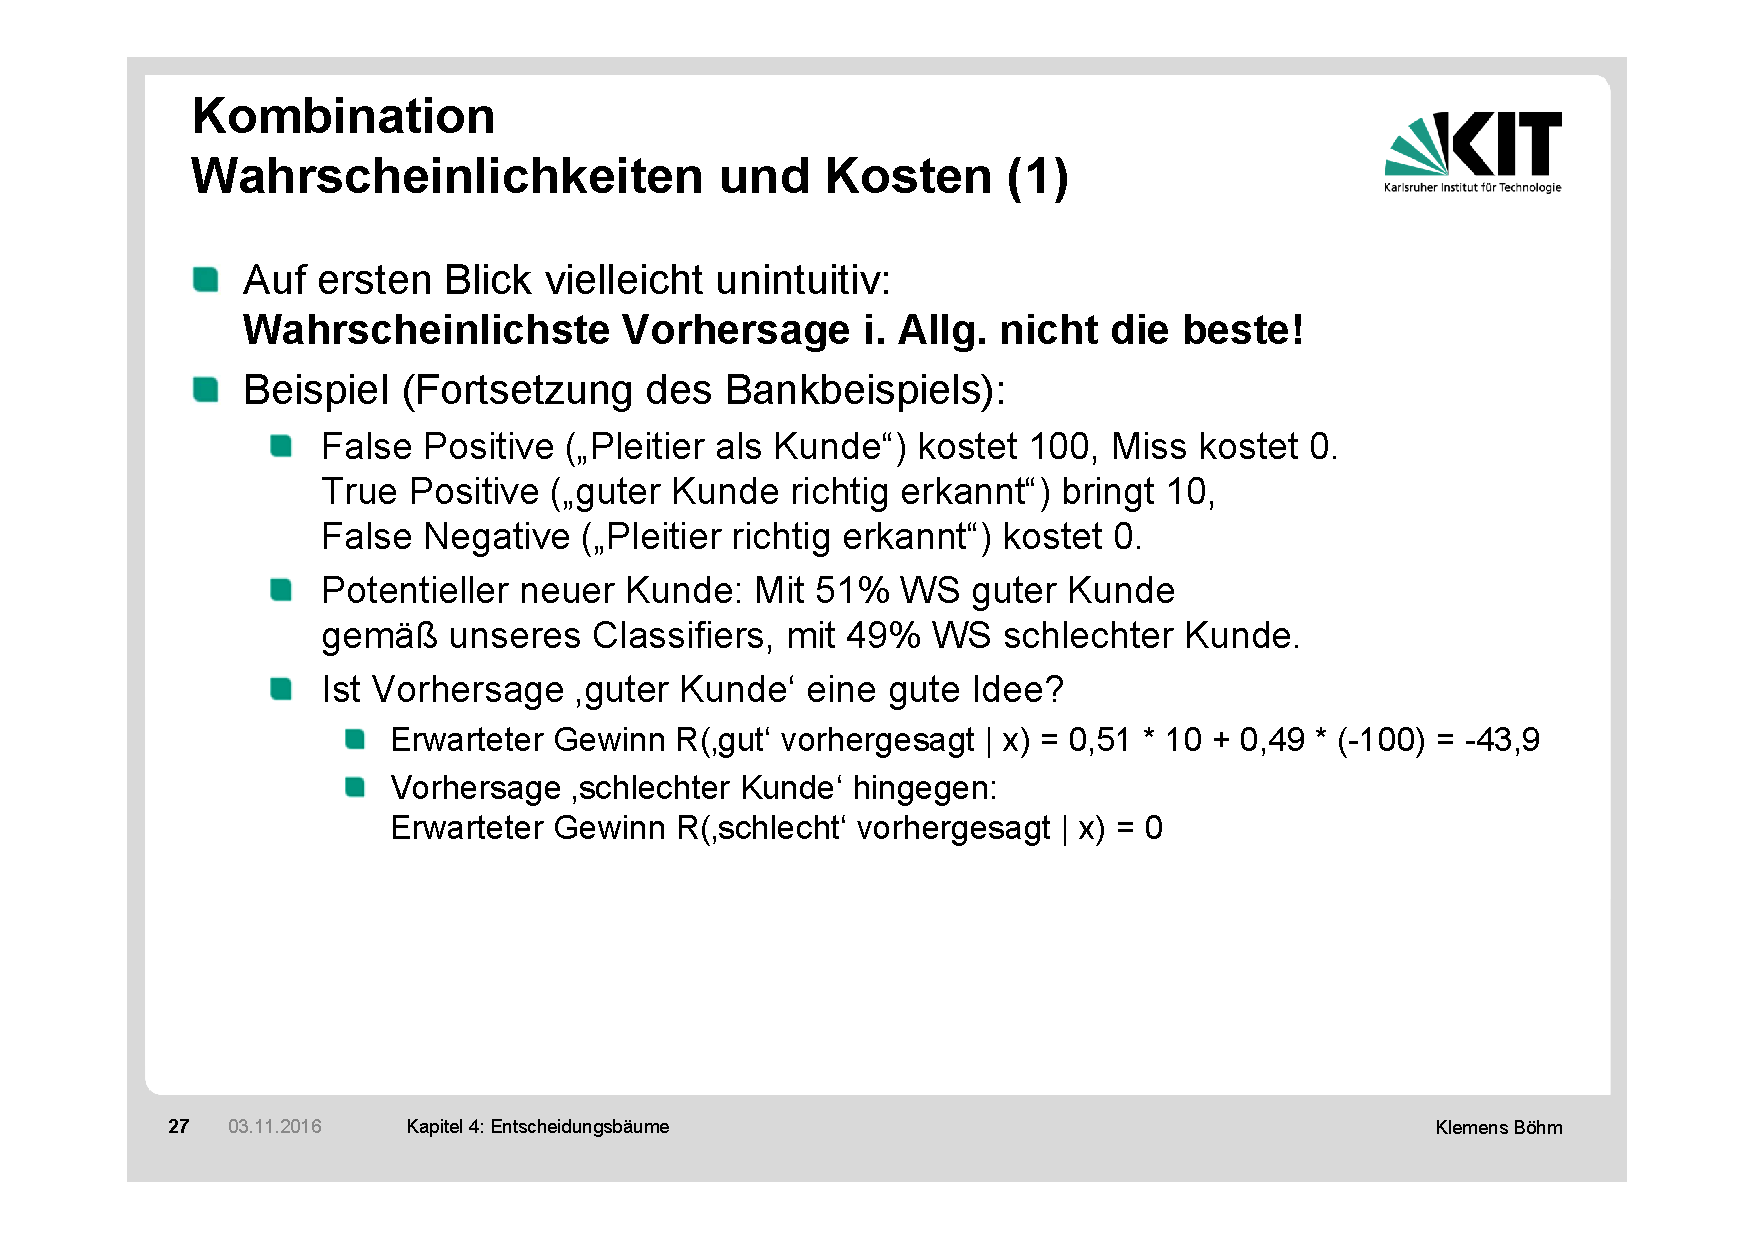
\includegraphics[width=0.75\textwidth]{Figures/classifier}
	\caption[Beispiel Classifier]{Beispiel für  den Fall, dass
	die wahrscheinlichste Vorhersage nicht auch die geringsten Kosten
	mit sich bringt.\footnotemark}
	\label{fig:classifier_ex}
\end{figure}
\footnotetext{4. Foliensatz, S. 27, Analysetechniken für große Datenbestände, Prof. Dr.-Ing. Klemens Böhm}

In Abb.~\ref{fig:classifier_ex} lässt sich dies gut nachvollziehen. Damit kann
man die Kosten und Wahrscheinlichkeiten in einer Formel miteinander verbinden
zu dem \textit{Conditional Risk}
\[
	R(i \mid x) = \sum_j P(j \mid x) \cdot Cost(i,j),
\]
wobei \(j\) die tatsächliche Klasse und \(i\) die vorhergesagt Klasse beschreibt.


\subsection{NULL-Werte}
NULL-Werte können von besonderer Bedeutung für die Analyse der Daten sein. So
kann ein fehlender Eintrag des Abiturdatums bedeuten, dass der Probant keine
höhere Bildung genossen hat. Es kann also nützlich sein, eine Unterscheidung auch
für NULL-Werte einzuführen. Bei der Erstellung des Baumes werden bei den
Splitkriterien die Werte, die in dem abgefragten Attribut einen NULL-Wert haben
gewichtet die jeweiligen Teilbäume hinabgeschickt und gehen dann damit am Ende auch
nur gewichtet in die Entscheidungen in den jeweiligen Blättern ein. Diese Gewichtung
geschieht entsprechende der Anzahl der Objekte, die einen Wert in dem Attribut vorweisen
und nach links bzw. rechts absteigen, also sind die beiden Gewichte für die 
NULL-Objekte \(\frac{n_1}{n_1 + n_2}\) und \(\frac{n_2}{n_1 + n_2}\).
